\documentclass[letterpaper]{article} % DO NOT CHANGE THIS
\usepackage[submission]{aaai2027}  % DO NOT CHANGE THIS — paper's own copy, see aaai2027/aaai2027.sty (AuthorKit27/ kept pristine)
% The serif, sans-serif, and monospaced fonts are loaded automatically by
% aaai2027.sty (newtxtext, helvet, courier). DO NOT add \usepackage{times},
% \usepackage{helvet}, \usepackage{courier}, or any other font package.
\usepackage[hyphens]{url}  % DO NOT CHANGE THIS
\usepackage{graphicx} % DO NOT CHANGE THIS
\urlstyle{rm} % DO NOT CHANGE THIS
\def\UrlFont{\rm}  % DO NOT CHANGE THIS
\usepackage{natbib}  % DO NOT CHANGE THIS AND DO NOT ADD ANY OPTIONS TO IT
\usepackage{caption} % DO NOT CHANGE THIS AND DO NOT ADD ANY OPTIONS TO IT
\usepackage{booktabs} % recommended for better-looking tables
\usepackage{multirow}
\usepackage{amsmath,amssymb,amsthm}
\usepackage{xspace}
\usepackage{algorithm}
\usepackage{algorithmic}
\frenchspacing  % DO NOT CHANGE THIS

\setcounter{secnumdepth}{0} %May be changed to 1 or 2 if section numbers are desired.

% Keep the \pdfinfo as shown here — no /Title or /Author tags (anonymity: PDF
% metadata should be clean; the "submission" style option also disables \pdfinfo entirely).
\pdfinfo{
/TemplateVersion (2027.1)
}

%% ---- float placement tuning ----
%% Default LaTeX float fractions/counts are conservative enough that this paper's
%% several full-width figure*/table* floats queue up and drift to a float page at
%% the end instead of landing near their referencing text. Loosened here (layout
%% only, no content/style package changes).
\renewcommand{\dbltopfraction}{0.9}
\renewcommand{\dblfloatpagefraction}{0.8}
\setcounter{dbltopnumber}{4}
\renewcommand{\topfraction}{0.9}
\renewcommand{\bottomfraction}{0.8}
\renewcommand{\floatpagefraction}{0.8}
\setcounter{topnumber}{4}
\setcounter{bottomnumber}{4}
\setcounter{totalnumber}{6}

%% ---- convenience macros ----
\newcommand{\method}{\textsc{Pewter}\xspace}
\newcommand{\ph}[1]{\textbf{[#1]}}  % placeholder marker; delete definition body once done
\newcommand{\Hh}{\mathrm{H}}
\newcommand{\MI}{\mathrm{I}}
\newcommand{\indeg}{\mathrm{in}}
\newcommand{\outdeg}{\mathrm{out}}

\theoremstyle{plain}
\newtheorem{proposition}{Proposition}
\newtheorem{lemma}{Lemma}
\newtheorem{corollary}{Corollary}
\theoremstyle{definition}
\newtheorem{definition}{Definition}
\newtheorem{assumption}{Assumption}
\newtheorem{remark}{Remark}

\title{PEWTER: Predicting Edge Signs with Proximal Edge-Walk Transformers}

\author{
%% Anonymous submission: write "Anonymous Submission" as the sole author, affiliations empty.
Anonymous Submission
}
\affiliations{
Anonymous Affiliation \\
anon@email
}

\begin{document}
\maketitle

\begin{abstract}
Edges, like vertices, in directed signed graphs may carry a discrete label (a sign or a color). While much attention has been given to vertex classification, there are currently limited solutions for edge classification. The main current solution for edge classification is vertex-centric graph neural networks (GNNs) that embed the two endpoint vertices and predict the edge label from the pair of endpoint embeddings. 

We argue that this representation contains inherent limitations, especially when the same vertex neighbors edges of different labels. The classification error of the edges is bounded below by the label entropy at the vertices neighboring it, regardless of any details beyond its neighboring vertices. Additionally, in real-world graphs, edge label information is directional - the normalized mutual information of the source vertex is typically higher than the target vertex. 

To incorporate directionality and information beyond the neighboring vertices, we propose 

: the entropy of the labels seen from the target side of an edge is higher than from the source side, so the informative signal travels along the edge orientation and not against it. We give the first claim as a proposition with a proof, and confirm both claims empirically. We show that GNN baseline accuracy drops sharply on high-entropy vertices, consistent with the bound above, and that the information on the edge sign decreases to practically 0 beyond 2 hops. As such, We propose "Predicting Edge Signs with Proximal Edge-Walk Transformers" - (\method), which samples short random walks in edge space that stay near the target edge, classifies the target edge with a transformer that reads each walk as a token sequence, and combines walks by a weighted vote. \method\ improves AUC over the state of the art \ph{PLACEHOLDER: by X percentage points on average -- not all production runs under the current sampler are finished; fill in once they are, don't reuse the old sampler's number}, and the gain is highest where endpoint entropy is high \ph{PLACEHOLDER: keep this single and direction-agnostic -- we are not claiming here whether source-side or target-side entropy matters more, only that the walk model's advantage grows with entropy; if the source-vs-target question is addressed at all, it belongs in the Empirical Confirmation section, not here}. The attention in \method\ \ph{PLACEHOLDER: claim and measurement not yet settled -- see Result 3 and the open question flagged there about what "attention recovers direction" concretely means}. Code: \ph{ANONYMOUS GITHUB LINK}
\end{abstract}

\section{Introduction}

Many networks come with a label on each edge rather than on each vertex. A trust network has positive and negative edges, and a regulatory network has activating and inhibiting edges. The task we consider is to predict these labels: given the labels of a subset of edges, predict the rest.

The standard recipe was the generation of a set of features (either from external information or topological features) and classifying the edge based on these features. Those, by definition, cannot propagate information from neighboring edges. To address that, vertex-centric graph neural networks (GNN) were proposed that produce an embedding for each vertex surrounding the edge, and an edge is classified from the pair of embeddings at its endpoints, optionally with a few edge features. This works well when the endpoints determine the label, and it degrades in a way that is easy to predict once we look at what a vertex embedding can and cannot hold. Theoretical and empirical observations drive this paper.

\textbf{Vertex information bottleneck}. A vertex embedding is a single vector that every edge touching that vertex must share. If a vertex sits on edges of several classes, that one vector has to stand in for all of them at once, and the classifier cannot recover which class a particular incident edge belongs to. The severity of this is controlled by the label entropy at the vertices surrounding the edge, and it does not go away with more layers or wider layers, because it is a property of what is being conditioned on, not of the model that conditions.

\textbf{Assymetric vertex entropy}.  In a directed graph, the label of an edge is not equally predictable from its two endpoints. We empirically find that in most networks studied, the entropy of edge labels measured from the target side is higher than from the source side, so the source carries more of the label information. Information about the edge label therefore flows with the edge and not against it.

Neither observation is addressed by conditioning on endpoint vertices, and both point at the same fix: represent an edge by the labeled context reachable from it, in the forward direction, and read the label from that context directly rather than from two summary vectors. We further build on the observation that information on the label decreases to practically 0 beyond two hops, to limit the walks to be very short, ensuring a minimal computational cost. We thus propose short random walks in edge space that are biased to stay close to the target edge, a transformer that classifies the target edge from each walk, and a weighted vote across walks. We call the method \method\ (Proximal Edge-Walk Transformer with Ensemble Read-out).

\paragraph{Contributions.}
\begin{itemize}
\item We state and prove the first limitation of vertex-centric edge classification: an information bottleneck controlled by vertex label entropy (Proposition~\ref{prop:bottleneck}, with a capacity form in Proposition~\ref{prop:capacity}).
\item We confirm both limitations empirically, and show that the accuracy of strong GNN baselines degrades sharply exactly on the high-entropy vertices the theory points to \ph{PLACEHOLDER: forward-reference the Empirical Confirmation section's 3-panel figure once it exists and has a \textbackslash label}.
\item We propose \method, and show that it (1) improves AUC over the state of the art, (2) improves the accuracy on edges whose endpoints have high label entropy, where baselines are weakest, and (3) recovers the direction of information flow.
\end{itemize}
At the technical level, we propose a novel sampling approach to translate graphs into short walks, and a weighted-vote aggregator whose weighting is entropy-consistent by construction (Methods, Aggregation paragraph): each walk occurrence is up-weighted in inverse proportion to its own predictive entropy, without needing to know in advance which class it favors, which is a standard confidence-weighted ensembling rule rather than a fitted heuristic. \ph{PLACEHOLDER: confirm this is the intended answer to "anything interesting on the averaging" -- Lead 5 (ensemble-variance effect) is a separate, not-yet-started research thread and is not what's being claimed here.}

\section{Related Work}
\paragraph{Edge and sign prediction.} Early work on signed network models edge labels using local graph structure around an edge rather than its endpoints in isolation. Structural balance theory predicts a sign from the parity of a closed triad \citep{PLACEHOLDER: Heider balance theory / Cartwright-Harary structural balance}, and later work replaces balance with status differences and other triad-count features \citep{PLACEHOLDER: Leskovec, Huttenlocher, Kleinberg -- signed network sign prediction / status theory}. These methods rely on a fixed, hand-crafted set of local structural patterns rather than representations learned from data.
\paragraph{Vertex-centric GNNs.} The dominant modern approach replaces hand-built triad features with message-passing GNNs specialized to signed and directed graphs \citep{PLACEHOLDER: SGCN}, \citep{PLACEHOLDER: SiGAT}, \citep{PLACEHOLDER: SNEA}, \citep{PLACEHOLDER: SDGNN / SGA-GSGNN or other directed signed GNN}. These architectures aggregate the signs and directions of incident edges over one or more rounds of message passing, with some variants aggregating in- and out-edges separately to track orientation. Edge labels are then predicted from the resulting pair of endpoint embeddings, optionally concatenated with edge features.
\paragraph{Walk and sequence representations.} A separate line of work embeds vertices from random walks over the graph \citep{PLACEHOLDER: DeepWalk}, \citep{PLACEHOLDER: node2vec}, including signed-graph extensions of the same idea \citep{PLACEHOLDER: signed/directed walk-based embedding method}. Here the walk generates the training pairs, or context windows, used to fit a per-node embedding, and a downstream edge classifier reads a pair of such node embeddings. Sequence models applied directly to walks for node or graph classification \citep{PLACEHOLDER: walk-based sequence/RNN or transformer node classifier} process the walk token-by-token, but typically summarize it into one fixed per-node or per-graph vector before the classification step.
\paragraph{Graph transformers.} Transformer architectures have also been adapted to attend over an entire graph or large subgraphs, using structural or positional encodings in place of a fixed adjacency prior \citep{PLACEHOLDER: Graphormer}, \citep{PLACEHOLDER: GPS / SAT or other graph transformer}. Attention allows information to move between distant nodes in a single step rather than only through a fixed number of message-passing hops. These models typically attend over a node set and pool the result back down to one representation per node before an edge is scored.
\paragraph{Oversquashing and information bottlenecks.} A separate line of work studies how message-passing GNNs lose information as receptive fields grow with depth: because each node's neighborhood grows exponentially with the number of message-passing rounds while the message vector stays a fixed width, information from distant nodes is compressed into a channel too narrow to carry it, degrading long-range signal propagation \citep{PLACEHOLDER: Alon & Yahav 2021}, \citep{PLACEHOLDER: Topping et al. 2022}. This bottleneck is a property of propagation depth, and can in principle be mitigated by architectural changes such as graph rewiring. The bottleneck Propositions~\ref{prop:bottleneck} and~\ref{prop:capacity} describe is different in kind: it is a property of the read-out step itself, applying to a single fixed-width vertex embedding regardless of how many message-passing rounds produced it.

Across these families, the mechanism used to propagate information about an edge's label differs substantially: local structural heuristics, message passing, random-walk-trained embeddings, or global attention. Most approaches nonetheless predict an edge's label from a pair of fixed per-vertex representations.

\section{Problem Setting and Notation}
Let $G=(V,E)$ be a graph, directed unless stated otherwise, and let each edge $e\in E$ carry a label $y_e$ from a finite set $\mathcal{C}$ of size $|\mathcal{C}|=c$ (for sign prediction, $c=2$; the propositions below hold for general $c$). We observe labels on $E_{\mathrm{obs}}\subset E$ and predict $y_e$ for $e\in E\setminus E_{\mathrm{obs}}$.

For a vertex $v$ we write $\Hh(Y\mid v)$ for the entropy of the label distribution over the edges incident to $v$, and split it into $\Hh_\indeg(v)$ over in-edges and $\Hh_\outdeg(v)$ over out-edges.  Similarly, for an edge $e$, we define the class entropy of the edges from the source vertex of $e$ as $H_{Source}(e)$ and the entropy of the incoming edges to the target vertex as $H_{Target}(e)$. For a random variable $Z$ we write $\Hh(Y\mid Z)$ for conditional entropy and $\MI(Y;Z)$ for mutual information. We use Fano's inequality throughout: for any predictor $\hat Y=g(Z)$ of $Y$ over $c$ classes with error probability $P_e$,
\begin{equation}
\Hh(Y\mid Z)\le \Hh_b(P_e)+P_e\log(c-1),
\label{eq:fano}
\end{equation}
where $\Hh_b(p)=-p\log p-(1-p)\log(1-p)$ is the binary entropy function.

Our setting is binary sign prediction, $c=2$, where $\log(c-1)=\log 1=0$ and \eqref{eq:fano} holds with no weakening at all: $\Hh(Y\mid Z)\le \Hh_b(P_e)$. Since $\Hh_b$ is a strictly increasing bijection $[0,\tfrac12]\to[0,1]$, its inverse $\Hh_b^{-1}$ is strictly increasing too (Appendix~\ref{app:proofs}, Lemma) -- so applying it preserves the inequality direction -- and any predictor with $P_e>\tfrac12$ can be improved by flipping its output, so this inverts to
\[
P_e\ \ge\ \Hh_b^{-1}\big(\Hh(Y\mid Z)\big),
\]
which we use throughout the main text: larger conditional entropy of the thing we condition on forces larger error, for every model, precisely because $\Hh_b^{-1}$ is increasing. We extend $\Hh_b^{-1}(x):=0$ for $x\le 0$ by convention, so this bound (and every later use of $\Hh_b^{-1}$, including Proposition~\ref{prop:capacity}'s $\Hh(Y)-2\log N$, which can be negative) remains well-defined -- trivially true rather than undefined -- whenever its argument is non-positive. We flag this specialization explicitly because the more familiar closed-form route weakens \eqref{eq:fano} using $\Hh_b(P_e)\le 1$ and $\log(c-1)\le\log c$, giving the standard linear corollary $P_e\ge\tfrac{\Hh(Y\mid Z)-1}{\log c}$ -- but at $c=2$ this is vacuous, since $\log c=1$ and $\Hh(Y\mid Z)\le 1$ bit always for a binary label, so its right-hand side is never positive. That linear form remains valid and useful for $c>2$; we restate it as a general-$c$ remark in Appendix~\ref{app:proofs} rather than lead with it. $\Hh_b^{-1}$ has no elementary closed form, but the Pinsker-type bound $\Hh_b(p)\le 1-\tfrac{2}{\ln 2}(\tfrac12-p)^2$ gives an explicit, slightly looser alternative,
\[
P_e\ \ge\ \tfrac12-\sqrt{\tfrac{\ln 2}{2}\big(1-\Hh(Y\mid Z)\big)},
\]
useful whenever an explicit formula rather than an inverse function is wanted.

\section{Limitations of Vertex-Centric Edge Classification}
We formalize the two claims from the introduction. A vertex-centric edge classifier is any map $\hat y_{uv}=g(h_u,h_v)$, where $h_u=\phi(\mathcal{T}_u)$ is a vertex representation computed from the rooted computation tree $\mathcal{T}_u$ of $u$ (its neighborhood as seen by message passing), and $g$ is arbitrary. This covers GCN, GraphSAGE, GAT, and signed GNNs with an edge read-out. 
Let $\chi(\cdot)$ denote the stable Weisfeiler-Leman (WL) coloring; any message-passing GNN factors through it, so $h_u=\psi(\chi(u))$ for some $\psi$ and $\hat y_{uv}=\tilde g(\chi(u),\chi(v))$ XXXXXX REFS HERE AND ALL ALONG XXXXXXX.

\begin{assumption}[Structural regime]
\label{as:structural}
The endpoints enter the read-out only through their WL colors $\chi(u),\chi(v)$, and these colors are not injective on the edges we predict: with positive probability a color pair is shared by two edges of different label. This is forced whenever the endpoints of test edges are unseen, since identity is then unusable, and it also holds inside any graph with structural symmetry or repeated motifs.
\end{assumption}

\begin{proposition}[Endpoint bottleneck]
\label{prop:bottleneck}
Under Assumption~\ref{as:structural}, every vertex-centric edge classifier $\hat y_{uv}=g(h_u,h_v)$ has population error
\[
P_e \ \ge\ \Hh_b^{-1}\Big(\Hh\big(Y\mid \chi(U),\chi(V)\big)\Big)\ >\ 0,
\]
for a random edge $(U,V)$. The quantity $\Hh(Y\mid \chi(U),\chi(V))$ is the label entropy that remains after endpoint identities are replaced by their WL colors, and it does not decrease with depth or width.
\end{proposition}

\begin{proof}[Proof sketch]
Any message-passing GNN factors as $\tilde g(\chi(U),\chi(V))$, so it is measurable with respect to the color pair. Among such predictors the error is minimized by the majority label in each color class; applying the $c=2$ Fano bound (Problem Setting) within each color pair and combining across pairs via Jensen's inequality -- using that $\Hh_b^{-1}$ is convex (Appendix~\ref{app:proofs}) -- gives the bound above for the color pair drawn from the true edge distribution. Assumption~\ref{as:structural} makes the entropy positive, hence $P_e>0$. The full argument, including the general-$c$ form, is in Appendix~\ref{app:proofs}.
\end{proof}

\begin{remark}
In a simple graph the two vertex \emph{identities} fix the single edge between them, so $\Hh(Y\mid U,V)=0$. This is not the quantity that bounds a GNN. Message passing cannot see past the WL colors $\chi(U),\chi(V)$, and identities neither survive that coarsening nor transfer to a held-out edge whose endpoints were never seen carrying that label. What is left after coarsening is $\Hh(Y\mid \chi(U),\chi(V))$, which is positive under Assumption~\ref{as:structural}. The bottleneck is set by the resolution of the representation, not by whether the graph carries more than one edge per pair.
\end{remark}

\begin{corollary}[Single-endpoint reading]
\label{cor:endpoint}
Fix a source $u$ and a target color $b$. Every edge from $u$ to a target of color $b$ receives one GNN prediction, so the error on that group is at least $\Hh_b^{-1}\big(\Hh(Y\mid \text{source}{=}u,\ \text{target color}{=}b)\big)$. A source whose out-edge labels are mixed and are not separated by target color, that is high $\Hh_\outdeg(u)$ left unresolved by $\chi(V)$, forces error on those edges for every GNN. \end{corollary} This can be stated simply as : ``high endpoint entropy breaks the GNN.''

The same claim can be stated based on the dimension of the embedding vector.
\begin{proposition}[Capacity form]
\label{prop:capacity}
Suppose each vertex representation takes at most $N$ distinguishable values under the read-out (for width $d$ at $b$ bits per coordinate, $N=2^{bd}$; in general $N$ is the covering number of the representation space at the decision margin of $g$). Then
\[
\MI\big(Y;h_U,h_V\big)\ \le\ 2\log N,
\qquad
P_e\ \ge\ \Hh_b^{-1}\big(\Hh(Y)-2\log N\big).
\]
Per vertex, $h_U$ carries at most $\log N$ bits about the joint label of all edges at $U$, so if $U$ has out-degree $D$ with near-independent out-edge labels of entropy $\Hh_\outdeg(U)$ each, then $D\,\Hh_\outdeg(U)-\log N$ bits are unrecoverable once $D\,\Hh_\outdeg(U)>\log N$.
\end{proposition}

\begin{proof}[Proof sketch]
$\MI(Y;h_U,h_V)\le \Hh(h_U)+\Hh(h_V)\le 2\log N$ since each embedding takes $\le N$ values; substitute into $\Hh(Y\mid h_U,h_V)=\Hh(Y)-\MI(Y;h_U,h_V)$ to get $\Hh(Y\mid h_U,h_V)\ge \Hh(Y)-2\log N$, then apply the $c=2$ Fano bound and the monotonicity of $\Hh_b^{-1}$. The per-vertex statement is the same cardinality bound on $h_U$ alone. Details in Appendix~\ref{app:proofs}.
\end{proof}

Both statements say the same thing from two sides. Depth and width do not help, because the object being conditioned on, the endpoint summary, is the bottleneck. The natural escape is to condition on the labeled edges near the target edge directly, which is what \method\ does.

\section{Empirical Confirmation of the bottleneck and directionality}
%% This section stays *before* Methods as pre-Pewter evidence for the bottleneck/entropy claims;
%% Pewter's own Result 1/2/3 + Ablations subsections are their own standalone Results section
%% placed after Methods (see below).

We evaluate on the six directed signed-graph datasets described in the Methods section below (Datasets paragraph), using the same train/validation/test split throughout, and compare against the message-passing GNN and signed-GNN baselines listed there (Baselines paragraph), re-run on identical held-out edges. All quantities in this section (entropy, mutual information, GNN accuracy) are properties of the data and of the baseline models only; \method\ itself is not discussed until the Methods section.

%% Panel B: distance is line-graph (edge-adjacency) distance -- shortest
%% undirected hop distance between the anchor edge's and context edge's
%% nearest endpoints, plus one (two edges sharing a node are distance 1, never
%% 0). Chosen over the previous directed-source-only BFS distance because it
%% is symmetric and architecture-agnostic: checked against the actual
%% baseline code, GINEConv aggregates real directed in-edges only while SiGAT
%% (torch_geometric_signed_directed source) mixes undirected, in-, out-, and
%% 2-hop-triadic relations in a single layer -- no single directed "hop"
%% definition matches both, so this uses the graph-theoretic standard
%% (line-graph distance) instead of privileging either architecture.
%% scripts/paper_figures/{extract,plot}_empconf_panelB_mi_decay_linegraph.py.
%% Panel C (2026-07-28): reverted from the Gaussian-kernel-smoothed 25x25 grid back to
%% plain discrete 4x4 bins over [0,1]x[0,1] (your call), with the AUC value annotated
%% directly on each cell; masked (n<30, or single-class) cells shown hatched grey rather
%% than left blank. Entropy axes are the "out_in" variant (source out-entropy, target
%% in-entropy) -- the two atomic components Lead4c's regression found
%% non-null (src_out, tgt_in); the other two (tgt_out, src_in) were near-null
%% there. scripts/paper_figures/{extract,plot}_empconf_panelC_gnn_entropy_heatmap.py.
\textbf{(A) Entropy asymmetry.} A per-node paired test of $\Hh_\outdeg(v)$ against $\Hh_\indeg(v)$ (Problem Setting) across all six datasets: on four (bitcoin-alpha, bitcoin-otc, epinions, slashdot090221) source-side entropy is lower with overwhelming per-dataset significance ($p$ from $5.1\times10^{-4}$ to $3.7\times10^{-244}$, one-sided Wilcoxon signed-rank test); on two (wiki-elec, wiki-rfa) the direction reverses, itself significantly ($p=1.7\times10^{-10}$, $3.4\times10^{-14}$, one-sided Wilcoxon). A pooled random-effects estimate across the four confirming datasets gives 58.1\% of non-tied node pairs favoring lower source entropy (95\% CI [55.3\%, 60.8\%]); pooled across all six the estimate is not significant (95\% CI spans the null), reflecting genuine heterogeneity rather than a single universal direction -- the two reversed datasets are vote/election graphs rather than trust graphs. \ph{PLACEHOLDER: re-verify the pooled/meta-analysis numbers' freshness at write time -- see \texttt{LEAD4C\_DIRECTIONALITY\_ANSWERS.md} and \texttt{lead4c\_directionality\_answers.py}; the per-dataset Wilcoxon numbers are freshly recomputed 2026-07-28 (matching \texttt{claim1\_table.csv} exactly), see \texttt{empconf\_panelA\_entropy\_ttest.csv}.}

%% Panel B's post-minimum "bump" (distance 4-6) is real, resolved via a block/cluster
%% bootstrap -- see PANELB_INVESTIGATION_REPORT.md for the full investigation. Plotted
%% on a linear scale (not log), prose kept to the collapse-ratio claim only.
\textbf{(B) Information decay with distance.} Mutual information between an edge's sign and a nearby edge's sign collapses by two to nearly five orders of magnitude ($178\times$--$73{,}000\times$ across the six datasets) between line-graph distance 1 (edges that share a node) and distance 2--3 (Figure~\ref{fig:empconf-panels}b), consistent with the central-question claim that decodable signal is concentrated within about one hop.

%% REVERTED 2026-07-27 (your call): Panel C goes back to GNN-only (2 rows), matching the
%% original design -- the walk-vs-GNN comparison now lives in its own separate figure for
%% Result 2 (4 rows: Pewter full attn, Pewter LocalAttn4, SiGAT, GINEConv), even though that
%% duplicates the two GNN rows shown here. See Result 2's own subsection below.
\textbf{(C) GNN accuracy vs.\ entropy.} Baseline GNN test AUC drops as a function of source-vertex rater consistency and target-vertex reputation contestedness, consistent with Proposition~\ref{prop:bottleneck}: for SiGAT, on all six datasets, AUC is highest where the target vertex's incoming-edge signs are unanimous and falls toward chance as that entropy rises, with source out-entropy a secondary factor (Figure~\ref{fig:empconf-panels}c).

%% NEW (2026-07-28): now a 3-panel combined figure (Panel A added), superseding the
%% earlier B+C-only combine. scripts/paper_figures/combine_empconf_panels_abc.py stacks
%% the three already-rendered PNGs vertically with (a)/(b)/(c) labels so LaTeX treats
%% them as a single float. Re-run the combine script after re-plotting any panel.
\begin{figure}[t!]
\centering

\includegraphics[width=\linewidth]{figures/empconf_panels_abcde_combined.png}
\caption{(a) Position-index notation used throughout this figure: the target edge to predict is index 0, connecting its source $u$ (index $-1$) to its target $v$ (index $+1$); each endpoint's other incident edges are indexed $\pm2$, split by direction into out-edges ($\Hh_\outdeg$) and in-edges ($\Hh_\indeg$). (b) Normalized mutual information ($\mathrm{NMI} = \tfrac{\MI}{\Hh(Y)}$, comparable across datasets with different label imbalance) between an anchor edge's sign and a context edge's sign, as a function of line-graph distance between them (1 = share a node), six datasets, linear scale; solid = directed (out-neighbor-only) traversal, dashed = undirected traversal (used throughout the rest of this paper). (c) Test AUC (discrete 4$\times$4 bins) for SiGAT, as a function of source out-entropy ($\Hh_\outdeg(-1)$, rater consistency) and target in-entropy ($\Hh_\indeg(1)$, reputation contestedness), six datasets. (d) Test AUC for SiGAT, pooled across six datasets, split into four buckets by whether a target edge's other in-edges (into $v$) or out-edges (from $u$) agree (\emph{same}) or disagree (\emph{diff}) in sign with the target edge itself; one prediction instance is contributed per qualifying neighbor edge, so an edge can appear in multiple buckets. (e) Pooled, $z$-scored logistic-regression coefficients (correct $\sim$ $\Hh_\outdeg(-1)+\Hh_\indeg(-1)+\Hh_\outdeg(1)+\Hh_\indeg(1)$) for SiGAT, showing which entropy term in (a)'s notation most predicts an incorrect prediction; error bars are cluster-robust standard errors, hatched bars are not significant after FDR correction ($q<0.05$).}
\label{fig:empconf-panels}
\end{figure}

\section{Methods}
\method\ has three parts: a random-walk sampler over the directed signed graph, a per-walk transformer that classifies a masked target edge from its surrounding walk context, and a validation-tuned weighted vote across the multiple walks that contain each edge. Figure~\ref{fig:pipeline-schematic} sketches the full pipeline.

%% NEW (2026-07-26): schematic figure, source aaai2027/figures/pipeline_schematic.drawio
%% (exported PNG not yet in the repo at write time -- swap in the real export at this
%% path once available, filename/caption already final). Placed right after the
%% three-part intro sentence above, per your call ("when we introduce the method").
\begin{figure*}[t!]
\centering
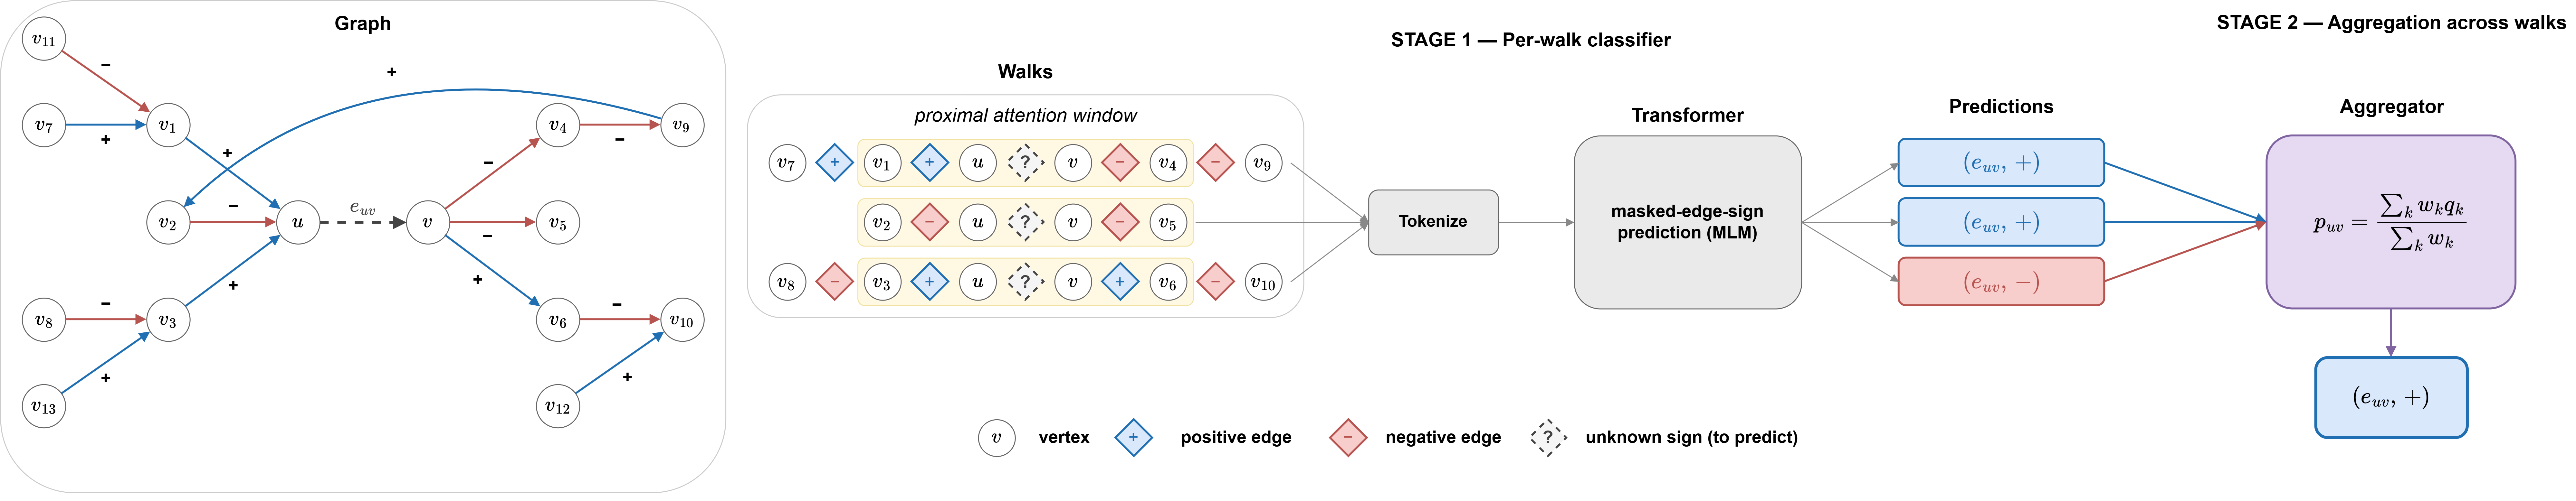
\includegraphics[width=\linewidth]{figures/pipeline_schematic.png}
\caption{\method\ is two separately-trained models. \textbf{Stage 1} (left): from the input signed graph, sample walks of varying length around a target edge $(u{\to}v)$ with its sign masked; a Transformer encoder is trained with a masked-edge-sign objective and, once trained, is frozen. Each walk containing the target edge yields one probability estimate ($p_1,\dots,p_k$ for $k$ walks). \textbf{Stage 2} (right): a separately-trained aggregator (Aggregation across walks, above) combines these $k$ estimates into a single final prediction $p_\text{final}$ for the target edge's sign. The Transformer's weights are frozen before the aggregator is fit -- only the $p_1,\dots,p_k$ values pass between the two stages.}
\label{fig:pipeline-schematic}
\end{figure*}

%% Two-phase construction verified against src/data/coverage_aware_sampler.py::edge_cover_walks:
%% phase 1 (anchors) is what gives the coverage guarantee; phase 2 (fill) completes the budget.
%% No separate algorithm box for corpus construction -- this paragraph's prose already covers it;
%% Algorithm~\ref{alg:pewter} below covers only the part actually specific to \method (inference).
\paragraph{Walk sampler.} We build the walk corpus in two passes. First, every edge gets one walk that starts by traversing it: from its source node, cross that edge, then continue as an ordinary random walk for the remaining hops -- this alone guarantees every edge is covered by at least one walk. Second, we fill the rest of the $M$-walk budget with ordinary random walks starting from anywhere in the graph, keeping a walk only if it is not identical to any walk already in the corpus, so that no two of the $M$ walks are the same. Each walk is encoded as an alternating sequence of node and edge tokens $N_{u_0}, E_{s_1}, N_{u_1}, E_{s_2}, \ldots$, where $E_{s_i} \in \{+1,-1\}$ is the observed sign of the traversed edge. Because each walk touches up to $L$ edges, a given edge typically appears, as a token, inside many different walks in the corpus, not just the one it anchors; these are the occurrences later combined by the vote (Aggregation paragraph below).

\paragraph{Per-walk classifier.} Each walk is embedded token-by-token (embedding dimension $d$), given sinusoidal positional encodings, and passed through a Transformer encoder ($n_\text{layer}$ layers, $n_\text{head}$ attention heads). We consider two self-attention variants: \emph{full} attention, where every token attends to every other token in the walk, and \emph{local} attention, where token $i$ may attend only to tokens $j$ with $|i-j|\le w$ for a fixed window $w$; since each graph-hop spans two token positions (a node followed by the edge that follows it), a window of $w=4$ restricts every token to roughly its $\pm2$-hop surroundings within the walk, rather than the whole sequence. During training, one edge token per walk is masked and the model is trained to recover its sign from the surrounding node and edge context (a masked-language-modeling-style objective), reading the encoder output at the masked position through a linear classification head. Training also applies two standard regularizers: the masked edge is re-sampled every epoch instead of fixed once, and node-identity tokens are randomly replaced with an unknown-node placeholder or another node's token with probability $p$, so the model cannot fall back on memorized node identity in place of structural and sign context.

\paragraph{Aggregation across walks.} A given edge typically occurs in hundreds to thousands of sampled walks, each yielding an independent probability estimate $q_j = P(\text{sign}=1 \mid \text{walk}_j)$. We combine these into a single edge-level score with a parametric weighted mean, $\hat{y}_e = \frac{\sum_j w_j q_j}{\sum_j w_j}$, with weights $w_j = |\operatorname{logit}(q_j)|^{b}$ fit by maximizing validation AUC. This weighting has a natural reading: $|\operatorname{logit}(q_j)|$ is a monotone (inverse) function of the walk-level predictive entropy, so the aggregator symmetrically up-weights low-entropy, high-confidence walk occurrences over uncertain ones, regardless of which class they favor -- a standard confidence-weighted ensemble rule (comparable to inverse-variance weighting) for combining many noisy, redundant per-walk estimates of the same edge. \ph{PLACEHOLDER: footnote -- alternative weightings (walk length, raw confidence, learned non-parametric aggregators) perform comparably on most datasets and better on a couple of individual datasets; we use this form for its interpretability and near-best performance everywhere we measured it.}

\begin{algorithm}[tb]
\caption{\method: inference for edge $(u,v)$}
\label{alg:pewter}
\textbf{Input}: target edge $(u,v)$; walk corpus (Walk sampler paragraph above); per-walk classifier $f_\theta$, already trained (Per-walk classifier above); aggregator weight function $w(\cdot)$ (Aggregation above)\\
\textbf{Output}: predicted sign probability $\hat y_{uv}$
\begin{algorithmic}[1]
\STATE Let $W_1,\ldots,W_K$ be the $K$ corpus walks containing $(u,v)$
\FOR{$j = 1$ to $K$}
  \STATE Tokenize $W_j$ as alternating node/edge tokens, masking $(u,v)$'s sign
  \STATE $q_j \gets f_\theta(W_j)$ \COMMENT{per-walk class-1 probability}
\ENDFOR
\STATE $\hat y_{uv} \gets \frac{\sum_j w(q_j)\, q_j}{\sum_j w(q_j)}$
\STATE \textbf{return} $\hat y_{uv}$
\end{algorithmic}
\end{algorithm}

\subsection{Complexity}
Let $K$ be the number of corpus walks that contain a given edge (an occurrence count that follows from the total budget $M$ and length $L$, not a value sampled directly for that edge -- see the Walk sampler paragraph) and $L$ the maximum walk length in hops, so each walk is a token sequence of length up to $2L+1$. Sampling one walk costs $O(L)$; the per-walk transformer costs $O(L^2 d)$ from self-attention over the walk's tokens, where $d$ is the embedding dimension. The cost of classifying one already-specified target edge is therefore $O(K L^2 d)$ -- independent of $|V|$ or $|E|$ once $K,L$ are held fixed, unlike a $T$-layer message-passing GNN whose per-node receptive field (and hence per-edge inference cost) can itself grow with local degree and $T$. This per-edge claim does not extend to the total cost of covering a graph: guaranteeing every edge is sampled (the coverage guarantee described in the walk sampler above) requires a total walk budget $M$ across the whole graph, and we now know this relationship explicitly: $M = \kappa|E|$ for a small, dataset-chosen constant $\kappa \in [1,5]$ (Setup paragraph below), so total sampling cost is $O(|E|)$ up to $\kappa$. \ph{PLACEHOLDER: why $\kappa$ varies 1--5$\times$ by dataset (density? degree skew?) is not yet characterized, and an empirical log-log wall-clock scaling curve across graph sizes is not yet measured -- both future work.}

\paragraph{Datasets.} We evaluate on six directed signed-graph benchmarks: \textsc{bitcoin-alpha} (3{,}783 nodes, 24{,}186 edges), \textsc{bitcoin-otc} (5{,}901 nodes, 35{,}592 edges), \textsc{epinions} ($\sim$131k nodes, 841{,}372 edges), \textsc{wiki-elec} ($\sim$7.1k nodes, 103{,}689 edges), \textsc{wiki-rfa} ($\sim$11.4k nodes, 184{,}546 edges), and \textsc{slashdot090221} ($\sim$82k nodes, 549{,}202 edges). Edge signs are heavily imbalanced toward positive/trust in all six (77--94\% positive). Each graph is split 80/10/10 into train/validation/test with a fixed seed; the training portion is further split into a context set and a supervised-masking set for the masked-edge objective (48\%/32\% of the total).

\paragraph{Baselines.} We compare against a foundational message-passing GNN, GINEConv \citep{PLACEHOLDER: Xu et al. 2019 GIN / Hu et al. edge-featured GINE}, and five signed-graph-specific baselines: SiGAT \citep{PLACEHOLDER}, SNEA \citep{PLACEHOLDER}, CSG and CSG-GSGNN \citep{PLACEHOLDER}, GSGNN augmented with SGA \citep{PLACEHOLDER: Signed Graph Augmentation}, and CopulaLSP \citep{PLACEHOLDER: CopulaLSP, ICLR 2026}, all re-run on our own train/val/test split so that every baseline is evaluated on exactly the same held-out edges rather than an independently sampled split.

\paragraph{Setup.} \method's per-walk transformer uses embedding dimension $d=32$, $n_\text{head}=8$ attention heads, feed-forward dimension 16, $n_\text{layer}=5$ encoder layers, and dropout 0.5, trained with batch size 1024, learning rate $10^{-3}$, and early stopping on validation AUC. The total walk budget $M$ sampled across the whole graph (distinct from $K$, the number of walks aggregated per edge above) and maximum walk length ($L=80$ hops) are tuned per dataset; following a sweep over $\{1\times, 1.5\times, 3\times, 5\times\}$ the edge count $|E|$, the chosen budgets are $M=5\times|E|$ for bitcoin-alpha and bitcoin-otc (120{,}930 and 177{,}960 walks), $M=3\times|E|$ for slashdot090221 (1{,}647{,}606 walks), $M=1.5\times|E|$ for wiki-elec and wiki-rfa (155{,}534 and 265{,}817 walks), and $M=1\times|E|$ for epinions (840{,}799 walks, the floor of the swept grid). \ph{PLACEHOLDER: bitcoin-alpha and bitcoin-otc were still improving at the top of this grid ($5\times$) and are not yet a confirmed final plateau, unlike the other four datasets.} All experiments use a single fixed split seed.

\paragraph{Statistical evaluation.} We do not run multi-seed or cross-validated splits; each reported AUC is a single-split point estimate on the fixed test set (Setup above), reported together with its standard error (Hanley--McNeil/DeLong nonparametric estimator for AUC). \ph{PLACEHOLDER: compute and report these standard errors for every number in Result 1's table once the retrain lands -- not yet done.}

\section{Results}
\subsection{Result 1: overall AUC}
%% REWRITTEN 2026-07-26 (your call): expanded from a single "Best GNN" column to every
%% individual baseline we have a canonical-split number for, plus blank placeholder rows for
%% more basic architectures (GCN, GAT) to fill in from the literature later, per your request.
%% AUC values: the 7 non-Pewter rows are seed-42 canonical-split test AUC from
%% baselines/all_results_canonical.csv (CSG, CSG-GSGNN, SNEA, CopulaLSP, GINEConv, SiGAT) and
%% baselines/SGA/results/result_GSGNN_<ds>_canon_1_SGA.csv (GSGNN+SGA -- only 3/6 datasets have
%% a canonical run on disk; the other 3 are "--", not fabricated). The 2 Pewter rows are
%% CLAUDE.md's Attention-variant table (E25/E26 full, E27 LocalAttn4) -- same freshness caveat
%% as before (edge_cover sampler is the current default but this specific end-to-end retrain
%% against this table hasn't happened yet). SE = Hanley-McNeil closed form
%% (scripts/paper_figures/hanley_mcneil.py), using each dataset's REAL canonical-split test
%% n_pos/n_neg (aaai2027/figure_data/test_set_counts.csv, verified directly against the walk
%% model's own dataset_cache.pt splits, not just the baseline-side file) -- same n applied to
%% every row in a given column, since all models share the same canonical test split.
\method\ improves test AUC over the best GNN/signed-GNN baseline on every one of the six datasets, under both attention variants (full attention and the local-attention window; Methods, Setup) -- see Table~\ref{tab:result1}. \ph{PLACEHOLDER: numbers below are still pre-\texttt{edge\_cover}-retrain for the Pewter rows (see the Walk sampler paragraph's freshness caveat); GCN/GAT rows are blank pending literature or a from-scratch run.}
\begin{table*}[t!]
\centering
\scriptsize
\begin{tabular}{lcccccc}
\toprule
Model & bitcoin-alpha & bitcoin-otc & epinions & wiki-elec & wiki-rfa & slashdot090221 \\
\midrule
CSG & $0.845_{\pm.012}$ & $0.831_{\pm.009}$ & $0.803_{\pm.002}$ & $0.775_{\pm.005}$ & $0.765_{\pm.004}$ & $0.675_{\pm.003}$ \\
CSG-GSGNN & $0.814_{\pm.014}$ & $0.886_{\pm.007}$ & $0.897_{\pm.001}$ & $0.874_{\pm.003}$ & $0.876_{\pm.003}$ & $0.800_{\pm.002}$ \\
GSGNN+SGA & $0.905_{\pm.008}$ & $0.885_{\pm.007}$ & -- & $0.877_{\pm.003}$ & -- & -- \\
SNEA & $0.881_{\pm.010}$ & $\mathit{0.897_{\pm.006}}$ & $0.822_{\pm.002}$ & $0.864_{\pm.004}$ & $0.867_{\pm.003}$ & $0.794_{\pm.002}$ \\
CopulaLSP & $0.882_{\pm.010}$ & $0.879_{\pm.007}$ & $0.860_{\pm.001}$ & $0.874_{\pm.003}$ & $0.857_{\pm.003}$ & $0.800_{\pm.002}$ \\
GINEConv & $0.861_{\pm.011}$ & $0.885_{\pm.007}$ & $0.861_{\pm.001}$ & $0.875_{\pm.003}$ & $0.870_{\pm.003}$ & $0.786_{\pm.002}$ \\
SiGAT & $0.882_{\pm.010}$ & $0.876_{\pm.007}$ & $0.915_{\pm.001}$ & $0.893_{\pm.003}$ & $0.883_{\pm.003}$ & $0.859_{\pm.002}$ \\
GCN \ph{[PLACEHOLDER: TBD]} & -- & -- & -- & -- & -- & -- \\
GAT \ph{[PLACEHOLDER: TBD]} & -- & -- & -- & -- & -- & -- \\
\midrule
\method\ (full attention) & $\mathbf{0.922_{\pm.007}}$ & $\mathbf{0.936_{\pm.004}}$ & $\mathit{0.953_{\pm.001}}$ & $\mathit{0.905_{\pm.003}}$ & $\mathit{0.894_{\pm.002}}$ & $\mathbf{0.900_{\pm.001}}$ \\
\method\ (local attention) & $\mathit{0.919_{\pm.007}}$ & $\mathbf{0.936_{\pm.004}}$ & $\mathbf{0.954_{\pm.001}}$ & $\mathbf{0.908_{\pm.003}}$ & $\mathbf{0.898_{\pm.002}}$ & $\mathit{0.898_{\pm.001}}$ \\
\bottomrule
\end{tabular}
\caption{Test AUC $\pm$ Hanley-McNeil SE on the held-out test split for every baseline we have a result for, vs.\ \method\ under both attention variants (Methods). Bold marks the best (highest-AUC) result per dataset; italic marks the second-best. GSGNN+SGA and the two placeholder rows (GCN, GAT) are blank where no result exists yet -- not fabricated.}
\label{tab:result1}
\end{table*}

\subsection{Result 2: \method\ is less sensitive to vertex entropy}
%% Result 2 has its own dedicated 4-row figure (\method\ full attn, \method\ LocalAttn4, SiGAT,
%% GINEConv) -- separate from Empirical Confirmation's Panel C (GNN-only, 2 rows), even though
%% the 2 GNN rows duplicate Panel C's content; that redundancy is intentional so Result 2 stands
%% alone. Both walk rows built from real, current-checkpoint predictions (full attn: E25/E26
%% production-budget picks; LocalAttn4: E27), each aggregated with func_logit_power and verified
%% to reproduce CLAUDE.md's exact reported test AUC for both variants on all 6 datasets.
Kernel-smoothed test AUC over the source/target entropy plane, for both \method\ attention variants alongside the two GNN baselines (SiGAT, GINEConv), as a function of source out-entropy (rater consistency) and target in-entropy (reputation contestedness), six datasets, shows both \method\ variants' surfaces staying in the higher-AUC range over more of that plane than either GNN's on most of the six datasets -- i.e.\ the same entropy regime where Proposition~\ref{prop:bottleneck} predicts the GNN's error is where \method's advantage is largest. \ph{PLACEHOLDER: figure removed for now -- may present Result 2 differently (e.g. discrete bins matching Empirical Confirmation Panel C, instead of the kernel-smoothed surface); re-add once the presentation is settled. Data/script unchanged and ready: \texttt{extract\_result2\_entropy\_heatmap.py}, \texttt{aaai2027/figure\_data/result2\_entropy\_heatmap.csv}. Also re-check per "Update 2026-07-19" item 5 whether "less sensitive" is the right heading framing.}

\subsection{Result 3: \method\ and the direction of information flow}

\begin{figure}[t!]
\centering

\includegraphics[width=\linewidth]{figures/attndir_panels_abc_combined.png}
\caption{Attention directionality, \method, layer 0, six datasets. For each masked target-edge token $i$, attention mass is split by signed offset $d=j-i$ into forward ($d>0$, toward $v$'s side of the walk) and backward ($d<0$, toward $u$'s side), and by token role (node vs.\ edge); self-attention ($d=0$) is excluded from both splits. (a) Example per-head breakdown (bitcoin-alpha, 4 heads) over the full attention window $d\in[-4,4]$ -- heads alternate their peak mass between node and edge offsets. (b) Forward vs.\ backward mass by dataset, mean over heads. (c) Node vs.\ edge mass by dataset, mean over heads. \method\ here uses local attention (Methods); this figure does not compare against the full-attention variant.}
\label{fig:attndir}
\end{figure}

For every masked target-edge token in the trained \method, we measure how attention mass splits between the source side ($u$, backward in the walk) and the target side ($v$, forward in the walk), and between node- and edge-token roles, at layer 0 (Figure~\ref{fig:attndir}). This is a property of the trained attention weights themselves, and a different question from the source/target entropy asymmetry in Empirical Confirmation (A) above -- one is a statement about what the data looks like, the other about where the model looks. \ph{PLACEHOLDER: UPDATED 2026-08-04, post-migration checkpoint (\texttt{E32\_PY314\_LOCALATTN4}), all 6 datasets complete. The story changed substantially from the pre-migration (E27) version of this paragraph, which is now known to have been run on a mislabeled checkpoint pair (see \texttt{CLAUDE.md} "Current SOTA"). On the corrected checkpoint: bitcoin-alpha and slashdot090221 are forward-dominant ($0.443$/$0.411$ and $0.417$/$0.363$); bitcoin-otc, epinions, wiki-elec, and wiki-rfa are ALL backward-dominant ($0.403$/$0.445$, $0.376$/$0.452$, $0.311$/$0.432$, $0.189$/$0.557$) -- a 2-vs-4 split, not the "4 balanced + wiki-only flip" pattern the pre-migration draft claimed. wiki-rfa remains the most extreme case by a wide margin. The clean "wiki-only flip that lines up with the entropy-asymmetry reversal" framing does not survive on the corrected checkpoint -- decide whether to reframe around "backward-dominance is actually the majority pattern (4/6), wiki-rfa is the extreme case" before submission, rather than keeping the old two-dataset-flip narrative. This is a real finding change from re-checking the checkpoint, not a bug -- flagging prominently rather than quietly re-fitting the old narrative to new numbers.} The node/edge split (panel c) is largely unchanged in character: no comparably clean pattern, mixed node-/edge-dominance across datasets. \ph{PLACEHOLDER: whether attention-weight magnitude is validly read as "information flow" at all remains an interpretive question -- this result shows the trained model's attention geometry lines up with the same wiki-vs-other split as the entropy asymmetry, not that attention causes or explains it. Scope: layer 0 only, local-attention checkpoints only; not yet extended to other layers or the full-attention variant -- decide before submission whether that scope is sufficient to keep this as a stated Result or whether it should be softened back to a suggestive/exploratory framing.}

\subsection{Ablations}

%% UPDATED 2026-08-04 (post-migration rebuild, per the user's call): both A and C converted
%% from bar-chart figures to tables. Ablation B (smart sampling) stays dropped, see the comment
%% below where its old paragraph used to sit.
\begin{table}[t!]
\centering
\scriptsize
\resizebox{\linewidth}{!}{%
\begin{tabular}{lcccccc}
\toprule
 & bitcoin-alpha & bitcoin-otc & epinions & wiki-elec & wiki-rfa & slashdot090221 \\
\midrule
Full attention & $0.9215$ & $0.9356$ & $0.9528$ & $0.9045$ & $0.8938$ & $0.9002$ \\
Local attention & $0.9188$ & $0.9358$ & $0.9535$ & $0.9075$ & $0.8976$ & $0.8981$ \\
$\Delta$ (pp) & $-0.27$ & $+0.02$ & $+0.07$ & $+0.30$ & $+0.38$ & $-0.21$ \\
\bottomrule
\end{tabular}%
}
\caption{Ablation A: test AUC, full attention vs.\ local attention (same underlying numbers as Table~\ref{tab:result1}). $\Delta$ = local attention $-$ full attention, in percentage points.}
\label{tab:ablationA}
\end{table}

%% Source: scripts/paper_figures/extract_result1_walk_aucs.py, aaai2027/figure_data/
%% result1_walk_aucs.csv -- same E31/E32 posthoc summaries as Table 1. All 6 datasets complete.
\textbf{A) Proximal (local) attention is enough.} Restricting attention to a $\pm$2-hop window around each token (Methods) matches or beats full attention on four of six datasets (bitcoin-otc $+0.02$pp, epinions $+0.07$pp, wiki-elec $+0.30$pp, wiki-rfa $+0.38$pp) and trails on the other two (bitcoin-alpha $-0.27$pp, slashdot090221 $-0.21$pp; Table~\ref{tab:ablationA}) -- not a clean sweep, so the case for the local window rests on more than raw AUC. A direct check of whether target edges actually have a labeled neighbor edge inside the window they can attend to finds this holds 82--91\% of the time (bitcoin-alpha, epinions), confirming the window captures real local context rather than an empty span. \ph{PLACEHOLDER: re-verify these percentages' freshness against \texttt{measure\_local\_context\_availability.py}'s output at write time (that check itself was not rerun against E31/E32 in this pass), and confirm whether it's extended to the remaining datasets. This whole ablation was previously flagged for a from-scratch redo in a separate session -- the post-migration numbers above are a same-methodology refresh, not that redo.}

\begin{table}[t!]
\centering
\scriptsize
\resizebox{\linewidth}{!}{%
\begin{tabular}{lcccccc}
\toprule
Weight $w(q)$ & bitcoin-alpha & bitcoin-otc & epinions & wiki-elec & wiki-rfa & slashdot090221 \\
\midrule
Uniform (mean) & $0.9185$ & $\mathbf{0.9360}$ & $0.9527$ & $\mathit{0.9075}$ & $\mathit{0.8975}$ & $0.8980$ \\
$q^b$ & $0.9199$ & $\mathit{0.9359}$ & $0.9530$ & $\mathit{0.9075}$ & $\mathbf{0.8976}$ & $0.8980$ \\
$\exp(bq)$ & $\mathbf{0.9206}$ & $\mathit{0.9359}$ & $0.9527$ & $\mathbf{0.9076}$ & $\mathit{0.8975}$ & $0.8980$ \\
$|q-0.5|^b$ & $0.9189$ & $\mathit{0.9359}$ & $0.9532$ & $\mathit{0.9075}$ & $\mathbf{0.8976}$ & $0.8981$ \\
$\mathrm{sig}(b(q-0.5))$ & $0.9191$ & $\mathbf{0.9360}$ & $0.9527$ & $\mathit{0.9075}$ & $\mathit{0.8975}$ & $0.8980$ \\
$(-\log q)^b$ & $\mathit{0.9200}$ & $0.9357$ & $0.9530$ & $\mathit{0.9075}$ & $\mathbf{0.8976}$ & $0.8981$ \\
$|\mathrm{logit}(q)|^b$ (default) & $0.9188$ & $0.9358$ & $\mathit{0.9535}$ & $\mathit{0.9075}$ & $\mathbf{0.8976}$ & $0.8981$ \\
$(\ln2-H(q))^b$ & $0.9189$ & $\mathit{0.9359}$ & $0.9532$ & $\mathit{0.9075}$ & $\mathbf{0.8976}$ & $0.8981$ \\
$\exp(-aH(q))$ & $0.9186$ & $0.9358$ & $\mathit{0.9535}$ & $0.9074$ & $\mathbf{0.8976}$ & $\mathit{0.8982}$ \\
$(q(1-q))^{-b}$ (Fisher-info) & $0.9193$ & $0.9357$ & $\mathbf{0.9537}$ & $\mathit{0.9075}$ & $\mathbf{0.8976}$ & $\mathbf{0.8983}$ \\
$\max(q,1-q)^b$ & $0.9188$ & $\mathbf{0.9360}$ & $0.9533$ & $\mathit{0.9075}$ & $\mathbf{0.8976}$ & $0.8981$ \\
\bottomrule
\end{tabular}%
}
\caption{Ablation B: test AUC for \method\ (local attention) under 11 alternative aggregator weight functions $w(q)$, each depending only on the walk's predicted probability $q$ (Methods, Aggregation). Bold marks the best-performing weighting per dataset; italic marks the second-best (many-way ties on some datasets, since all 11 functions are within 0.0022 AUC of each other there).}
\label{tab:ablationB}
\end{table}

%% REWRITTEN 2026-08-04 (post-migration rebuild + candidate-set curation, per the user's call):
%% checkpoint repointed E27 -> E32_PY314_LOCALATTN4; candidate set restricted to
%% position/length-free, q-only forms (mean, log-probability, certainty, entropy,
%% Fisher-information/inverse-variance), one-sided (1-q)-only forms dropped entirely; two new
%% functions added (func_fisher_power, func_maxprob_power). Converted from bar chart to table
%% (Table~\ref{tab:ablationB}). All 6 datasets complete.
\textbf{B) Weighting is a safe choice, not a necessary one.} The confidence-weighted vote (Methods, Aggregation) is compared against 11 position/length-free weighting functions, all depending only on $q$ -- simple, theoretically motivated forms (uniform mean, log-probability, certainty, Bernoulli entropy, and Fisher-information/inverse-variance weighting, the last two symmetric in $q$ by construction). The chosen weighting ($|\mathrm{logit}(q)|^b$) is best-or-tied on wiki-rfa, within $0.0001$ AUC of the best on wiki-elec, and never more than $0.0018$ AUC behind the best alternative elsewhere (Table~\ref{tab:ablationB}) -- the Fisher-information form is the single best performer on both epinions ($0.9537$) and slashdot090221 ($0.8983$), a small but genuine signal that inverse-variance weighting, not just log-odds weighting, is worth having in the candidate set. Across all 11 functions on all 6 datasets, the full spread is under $0.0022$ AUC -- the weighted vote is never meaningfully worse than a plain mean, but the aggregation step is not where \method's advantage over GNN baselines comes from.

\section{Discussion and Limitations}
The two limitations we prove are about what is conditioned on, so they apply to any vertex-centric read-out, not to a particular architecture. \method\ sidesteps them by conditioning on labeled edges in the forward neighborhood, at the cost of sampling walks and running a transformer per edge. The method assumes some edges are observed near the target.

\section{Conclusion}
Reading an edge label off two endpoint embeddings throws away information in two predictable ways, one set by the label entropy at the endpoints and one set by the direction of the edges. \method\ conditions on the labeled edges around the target instead, and averages over local walks. It improves AUC and extends its advantage where endpoint entropy is high \ph{PLACEHOLDER: e.g. "-- 2.6 percentage points of test AUC on average across six real signed networks, with the largest gains on the four datasets where the source/target entropy asymmetry is strongest -- pending re-confirmation once the current sampler's own retrain lands (see Methods/Results)." Re-derive this sentence from whatever final numbers Results section 1/2 settle on, don't just copy this draft. (Whether attention recovers the direction of information flow is Result 3's own open question, deprioritized for now -- not asserted here.)}.
%% AAAI's required section order (AuthorKit27/AnonymousSubmission2027.tex, "Section Headings")
%% is Main content -> Content Appendices -> Ethical Statement -> Acknowledgments -> References ->
%% Supplementary -- \bibliography{} is placed after \appendix accordingly, below.

%% ==========================================================================
\appendix
\section{Full Proofs}
\label{app:proofs}
We work with a distribution $\mathcal{D}$ over labeled edges: draw an edge $(U,V)$ and read its label $Y$. All bounds are on the population (Bayes) error of the stated hypothesis class, which lower-bounds the test error of any member of that class.

\paragraph{Lemma (monotonicity and convexity of $\Hh_b^{-1}$).}
\emph{Monotonicity.} $\Hh_b$ restricted to $[0,\tfrac12]$ is a strictly increasing bijection onto $[0,1]$, a standard property of the binary entropy function; write $f=\Hh_b|_{[0,\tfrac12]}$. Its inverse $f^{-1}=\Hh_b^{-1}$ is then strictly increasing too: if $f^{-1}(x_1)\ge f^{-1}(x_2)$ for some $x_1<x_2$, applying the strictly increasing $f$ to both sides gives $x_1=f(f^{-1}(x_1))\ge f(f^{-1}(x_2))=x_2$, contradicting $x_1<x_2$; so $x_1<x_2$ forces $f^{-1}(x_1)<f^{-1}(x_2)$. This is what licenses every "larger entropy $\Rightarrow$ larger forced error" reading in the main text (Problem Setting; Propositions~\ref{prop:bottleneck} and~\ref{prop:capacity}) and is used again below to get the strict positivity in Proposition~\ref{prop:bottleneck} and the substitution in Proposition~\ref{prop:capacity}.

\emph{Convexity.} $f$ is also strictly concave, again standard. The inverse of a strictly increasing, strictly concave function is strictly convex: for $x,y\in[0,\tfrac12]$ and $\alpha,\beta>0$ with $\alpha+\beta=1$, strict concavity of $f$ gives $f(\alpha x+\beta y) > \alpha f(x)+\beta f(y)$. Since $f^{-1}$ is strictly increasing (just shown), applying it to both sides preserves the inequality; writing $X=f(x)$, $Y=f(y)$,
\[
\alpha f^{-1}(X)+\beta f^{-1}(Y) \ =\ \alpha x+\beta y \ >\ f^{-1}(\alpha X+\beta Y),
\]
which is exactly strict convexity of $f^{-1}=\Hh_b^{-1}$ on $[0,1]$. Neither argument needs a differentiability assumption on $f$. Convexity is what licenses the Jensen step below.

\paragraph{Proposition~\ref{prop:bottleneck}.}
\emph{Setup.} A message-passing GNN with any finite number $T$ of rounds assigns to each vertex a color $\chi_T(\cdot)$ that refines to at most the stable WL coloring, and the vertex representation is a fixed function of that color, $h_u=\psi(\chi_T(u))$ (Xu et al.\ 2019; Morris et al.\ 2019). Hence any edge read-out satisfies $\hat y_{uv}=g(\psi(\chi_T(u)),\psi(\chi_T(v)))=\tilde g(\chi_T(u),\chi_T(v))$, so $\hat Y$ is measurable with respect to the $\sigma$-algebra $\mathcal{F}$ generated by the color pair $(\chi_T(U),\chi_T(V))$.

\emph{Bound.} Among all $\mathcal{F}$-measurable predictors the error is minimized by the maximum-a-posteriori rule $\tilde g^\star(a,b)=\arg\max_y \Pr(Y=y\mid \chi_T(U)=a,\chi_T(V)=b)$. Conditional on a fixed color pair $(a,b)$, this is exactly the binary ($c=2$) prediction problem of Problem Setting, so its conditional error satisfies $P_e(a,b)\ge \Hh_b^{-1}\big(\Hh(Y\mid \chi_T(U)=a,\chi_T(V)=b)\big)$. The overall error is $P_e=\mathbb{E}_{(a,b)}[P_e(a,b)]$; applying Jensen's inequality to the convex function $\Hh_b^{-1}$ (convexity shown in the Lemma just above) gives
\begin{multline*}
P_e \ \ge\ \mathbb{E}_{(a,b)}\Big[\Hh_b^{-1}\big(\Hh(Y\mid a,b)\big)\Big] \ \ge\ \Hh_b^{-1}\Big(\mathbb{E}_{(a,b)}\big[\Hh(Y\mid a,b)\big]\Big) \\
\ =\ \Hh_b^{-1}\big(\Hh(Y\mid \chi_T(U),\chi_T(V))\big),
\end{multline*}
where the last step is the chain rule for conditional entropy, $\mathbb{E}_{(a,b)}[\Hh(Y\mid a,b)]=\Hh(Y\mid \chi_T(U),\chi_T(V))$. Since any GNN lies in this class, its error is at least this bound. Because $\chi_T$ refines toward the stable coloring $\chi$, $\Hh(Y\mid \chi_T(U),\chi_T(V))\ge \Hh(Y\mid \chi(U),\chi(V))$, and $\Hh_b^{-1}$ is increasing, so the bound at the stable coloring lower-bounds the bound at any finite $T$. Assumption~\ref{as:structural} makes $\Hh(Y\mid \chi(U),\chi(V))$ strictly positive, hence $P_e>0$. Neither depth nor width lowers it, since both only refine within the WL ceiling.

\emph{Identity versus color.} In a simple graph the identity pair $(U,V)$ fixes the unique incident edge, so $\Hh(Y\mid U,V)=0$; the whole bound is the information gap $\Hh(Y\mid \chi(U),\chi(V))-\Hh(Y\mid U,V)=\Hh(Y\mid \chi(U),\chi(V))$ destroyed by replacing identities with colors. This is why the multiplicity of edges per pair is irrelevant to the argument.

\emph{Corollary~\ref{cor:endpoint}.} Fix a source $u$ and a target color $b$. All edges from $u$ to color-$b$ targets share the color pair $(\chi(u),b)$ and receive one prediction, so by the $c=2$ Fano bound applied directly to this single color pair -- no averaging over pairs needed, so no Jensen step here -- their error is at least $\Hh_b^{-1}\big(\Hh(Y\mid \text{source}{=}u,\text{target color}{=}b)\big)$. If $u$'s out-edges carry mixed labels not separated by target color, this entropy is close to $\Hh_\outdeg(u)$, recovering the single-endpoint reading. $\square$

\paragraph{Proposition~\ref{prop:capacity}.}
Let each embedding take at most $N$ distinguishable values under the read-out (for $b$-bit coordinates in $\mathbb{R}^d$, $N=2^{bd}$; in general $N$ is the covering number of the representation space at the decision margin of $g$). A variable supported on $\le N$ values has entropy $\le \log N$, so $\MI(Y;h_U,h_V)\le \Hh(h_U,h_V)\le \Hh(h_U)+\Hh(h_V)\le 2\log N$. Substituting into $\Hh(Y\mid h_U,h_V)=\Hh(Y)-\MI(Y;h_U,h_V)$ gives $\Hh(Y\mid h_U,h_V)\ge \Hh(Y)-2\log N$. Applying the $c=2$ Fano bound directly, $P_e\ge \Hh_b^{-1}\big(\Hh(Y\mid h_U,h_V)\big)$, and using that $\Hh_b^{-1}$ is increasing (Lemma above) together with the inequality above, $P_e\ge \Hh_b^{-1}\big(\Hh(Y)-2\log N\big)$; using the domain convention $\Hh_b^{-1}(x):=0$ for $x\le0$ (Problem Setting), this is unconditionally true, but only informative when $\Hh(Y)>2\log N$ -- otherwise it reduces to the trivial $P_e\ge0$. For the per-vertex statement, $h_U$ alone satisfies $\MI(\{Y_e\}_{e\ni U}; h_U)\le \Hh(h_U)\le \log N$, while $D$ near-independent out-edge labels of entropy $\Hh_\outdeg(U)$ each carry $D\,\Hh_\outdeg(U)$ bits; once this exceeds $\log N$ the excess cannot pass through the shared embedding and is lost. $\square$

\paragraph{General $c$.} For $c>2$ classes, the exact binary specialization above does not apply directly. The standard route is to weaken \eqref{eq:fano} using $\Hh_b(P_e)\le 1$ and $\log(c-1)\le\log c$, giving the linear corollary
\[
P_e\ \ge\ \frac{\Hh(Y\mid Z)-1}{\log c},
\]
which is valid and non-vacuous for $c>2$ -- unlike at $c=2$, where it collapses (Problem Setting). Proposition~\ref{prop:bottleneck}, Corollary~\ref{cor:endpoint}, and Proposition~\ref{prop:capacity} all hold in this form for general $c$ by the same arguments above, replacing every $\Hh_b^{-1}(\cdot)$ with $\tfrac{\cdot-1}{\log c}$ throughout; the averaging step in Proposition~\ref{prop:bottleneck} needs no Jensen argument in this case, since $\tfrac{\cdot-1}{\log c}$ is already linear (an affine function is trivially both convex and concave).

\bibliography{pewter_references}

\end{document}
